\chapter{Grundlagen}
\section{Machine Learning}
Machine Learning ist eine Unterkategorie der künstlichen Intelligenz und bezeichnet einen automatisierten Prozess, der es Computern ermöglicht, eigenständig aus Trainingsdaten zu lernen und sich mit der Zeit zu verbessern, ohne explizit zur Lösung einer Aufgabe programmiert zu werden.
Machine Learning Algorithmen können Muster in Daten entdecken und aus ihnen Lernen, um eigene Prognosen und Entscheidungen zu treffen.

In der Regel wird Machine Learning in folgende Teilbereiche untergliedert \cite{monkeylearnIntroductionMachine}:
\begin{itemize}
    \item \textbf{Supervised Learning:}
    Ein Modell wird anhand von gelabelten Trainingsdaten trainiert.
    Ein Datentupel besteht dabei aus einer Eingabe und der dazu gewollten Ausgabe.
    Der Algorithmus sucht beim Training nach Zusammenhängen und Abhängigkeiten um anschließend Ausgaben für unbekannte Eingaben generieren zu können.
    Üblicherweise wird Supervised Learning für Regressions- und Klassifikations-Probleme eingesetzt.

    \item \textbf{Unsupervised Learning:}
    Wird in der Regel für Clusterbildung von unbeschrifteten Trainingsdaten verwendet.
    Der Algorithmus muss dabei selbstständig nach Mustern in den Daten suchen.
    Unsupervised Learning kann dabei helfen, Einblicke in große Datensätzen zu erhalten, um etwa versteckte Trends zu entdecken.

    \item \textbf{Semi-Supervised Learning:}
    Für das Training werden beim Semi-Supervised Learning sowohl ein kleiner gelabelter, als auch ein großer ungelabelter Datensatz verwendet.
    Dabei werden die Vorzüge von Supervised und Unsupervised Learning miteinander verbunden.
    Interessant ist dies vor allem bei sehr großen Datensätzen (zum Beispiel bei Bild-Klassifizierung), da die Labelung der Daten in der Regel manuell erfolgen muss.

    \item \textbf{Reinforcement Learning:}
    Beim Reinforcement Learning kann ein Agent Aktionen tätigen, für die er entweder belohnt oder bestraft wird.
    Es ist sein Ziel, selbstständig ein bestmögliches Verhalten zu lernen, um seine Belohnung zu maximieren.
    Dabei werden keine Trainingsdaten verwendet.
    Der Agent lernt ausschließlich aus seinen eigenen Erfahrungen und Fehlern.
    Reinforcement Learning findet vor allem in den Bereichen Robotik und Videospiele Einsatz und wird auch in dieser Arbeit verwendet werden.
\end{itemize}

% \begin{itemize}
%     \item Unterkategorie der künstlichen Intelligenz
%     \item ML ist ein automatisierter Prozess, der ...
%     \item ermöglicht Computern, eigenständig aus Trainingsdaten zu lernen und sich mit der Zeit zu verbessern, ohne explizit programmiert zu werden
%     \item ML Algorithmen können Muster in Daten entdecken und aus ihnen lernen, um eigene Voraussagen und Entscheidungen zu treffen
    
%     \item verschiedene Teilbereiche
%     \item Supervised Learning
    
%     Vorhersagen von gelabelten Trainingsdaten
%     Datensatz: Input mit gewolltem Output
%     \item Unsupervised Learning
    
%     Einblicke und Beziehungen in unbeschrifteten Daten
%     Modelle müssen selbstständig Muster finden
%     Clustering
%     kann helfen, versteckte Muster oder Trends zu entdecken
%     \item Semi-Supervised Learning
    
%     kleiner Teil gelabelter Daten, viele ungelabelte
%     besonders für große Datensätze interessant, Bild-Klassifizierung
%     \item Reinforcement Learning
    
%     vor allem im Bereich Robotik und Videospiele vertreten
%     Agent kann Aktionen tätigen, für die er belohnt oder bestraft wird
%     es ist sein Ziel, ein bestmögliches Verhalten zu lernen, um seine Belohnung zu maximieren
%     keine Trainingsdaten, Lernen aus eigenen Fehlern
%     in diesem Kontext besonders interessant wird verwendet

%     \item \cite{monkeylearnIntroductionMachine}
% \end{itemize}

\subsection{Reinforcement Learning}
Reinforcement Learning ist ein rechnerischer Ansatz, um zielorientierte Lern- und Entscheidungsprozesse zu verstehen und nachzubilden.
Wie oben schon beschrieben, steht dabei ein \emph{Agent} im Zentrum, der aus der direkten Interaktion mit seiner \emph{Umgebung (engl. Environment)} lernt, ohne dabei eine beispielhafte Anleitung oder vollständige Modelle der Umgebung zu benötigen.
Das formale Framework des \emph{\ac{mdp}} wird genutzt, um die Interaktion zwischen dem lernenden Agenten und seiner Umgebung zu definieren.
\acp{mdp} sind eine mathematisch idealisierte Form eines Reinforcement Learning Problems, für die präzise, theoretische Aussagen getroffen werden können \cite[13]{sutton2018rlintro}.
\autoref{fig:mdp} stellt die grundlegende Struktur eines Reinforcement Learning Problems dar.
Die einzelnen Bestandteile der Abbildung werden nachfolgend erläutert.

\begin{figure}
    \centering
    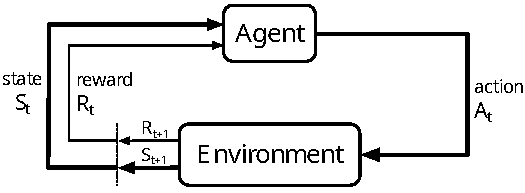
\includegraphics[width = 0.7\textwidth]{Bilder/MDP.pdf}
    \caption{Die Interaktion von Agent und Umgebung als \ac{mdp} \cite[48]{sutton2018rlintro}}
    \label{fig:mdp}
\end{figure}

Agenten haben explizite Ziele, können Aspekte ihrer Umgebung wahrnehmen und \emph{Aktionen} $A$ auswählen, um mit ihrer Umgebung zu interagieren und diese zu beeinflussen.
Es wird davon ausgegangen, dass Reinforcement Learning diejenige Strategie des Machine Learning ist, die dem natürlichen Lernen von Menschen und Tieren am nächsten kommt.
Viele zentrale Algorithmen des Reinforcement Learnings sind ursprünglich durch biologische Systeme inspiriert \cite[4]{sutton2018rlintro}.

Besonders wichtig für Reinforcement Learning ist das Konzept von \emph{Zuständen} $S$.
Ein Zustand kann dabei als eine Art Signal verstanden werden, das dem Agent Informationen über den Zustand der Umgebung liefert.
Weiterhin definieren folgende Elemente ein Reinforcement Learning Problem:
\begin{itemize}
    \item \textbf{Policy} $\mathbf{\pi}$\textbf{:}
    Die Policy definiert, wie sich der Agent zu einer gegebenen Zeit verhält.
    Sie stellt ein Mapping zwischen den wahrgenommenen Zuständen der Umgebung und den durchzuführenden Aktionen dar.
    Die Policy ist hinreichend, um das Verhalten des Agent zu bestimmen \cite[6]{sutton2018rlintro}.

    \item \textbf{Reward-Signal} $\mathbf{R}$\textbf{:}
    Das Reward-Signal definiert das Ziel eines Reinforcement Learning Problems.
    Bei jedem \emph{Zeitschritt} $t$ sendet die Umgebung ein Skalar an den Agent.
    Das einzige Ziel des Agent ist die Maximierung des kumulativen Rewards.
    Der Reward ist die primäre Basis für Änderungen an der Policy \cite[6]{sutton2018rlintro}.

    \item \textbf{Value-Funktion} $\mathbf{V}$\textbf{:}
    Die Value-Funktion legt fest, was auf lange Sicht gut ist.
    Der Value eines Zustands ist der kumulierte Reward, den ein Agent, ausgehend von diesem Zustand, in der Zukunft erwarten kann.
    Values geben die langfristige Attraktivität von Zuständen an.
    Die Wahl einer Aktion wird auf Basis der Value-Einschätzung des aktuellen Zustands getroffen.
    Im Vergleich zum Reward-Signal sind Values allerdings deutlich schwerer zu bestimmen, da diese anhand einer Sequenz von Observationen des Agenten geschätzt werden müssen \cite[6]{sutton2018rlintro}.

    \item \textbf{Modell der Umgebung (optional):}
    Manche Reinforcement Learning Systeme nutzen ein Modell der Umgebung.
    Dieses Modell erlaubt das Ziehen von Schlussfolgerungen über das Verhalten der Umgebung.
    So kann etwa eine Voraussage des nächsten Resultierenden Zustands und Rewards, ausgehend von einem gegebenen Zustand und einer Aktion getroffen werden.
    Genutzt werden diese Modelle zur Planung.
    Es werden also Entscheidungen für eine Folge von Aktionen auf Basis möglicher zukünftiger Situationen getroffen, bevor diese tatsächlich erlebt werden.
    Reinforcement Learning Methoden, die Modelle und Planung verwenden, werden als \emph{modell-basiert} bezeichnet.
Im Gegensatz dazu stehen \emph{modell-freie} Methoden, welche explizit auf Basis von Trial-And-Error lernen \cite[7]{sutton2018rlintro}.
\end{itemize}

Beim Reinforcement Learning versucht der Agent, mit seinen ausgeführten Aktionen ein Reward-Signal zu maximieren.
Dabei muss ein Kompromiss zwischen Nutzen des Gelerntem und Entdecken von Neuem gefunden werden.
Es besteht das Dilemma, dass weder das eine, noch das andere uneingeschränkt verfolgt werden kann, ohne bei der Ausführung der Aufgabe zu scheitern, denn beim Entdecken muss der Agent auch schlechte Aktionen ausführen, für die er keinen Reward erhält.
Entdeckt er jedoch nichts, weiß er auch nicht, welche Aktionen einen hohen Reward erzeugen \cite[3]{sutton2018rlintro}.

% \begin{itemize}
%     \item Markov Decision Processes sind eine mathematisch idealisierte Form eines Reinforcement Learning Problems für die präzise theoretische Aussagen getroffen werden können
    
%     \item rechnerischer Ansatz, um zielorientierte Lern- und Entscheidungsprozesse zu verstehen
%     \item im Zentrum steht dabei ein Agent, der aus der direkten Interaktion mit seiner Umgebung lernt, ohne dabei eine beispielhafte Anleitung oder vollständige Modelle der Umgebung zu benötigen
%     \item nutzt das formale Framework des Markov Decision Processes um die Interaktion zwischen dem lernenden Agenten und seiner Umgebung zu definieren
%     \item Versuch, ein Reward-Signal zu maximieren
%     \item Kompromiss zwischen Nutzen und Entdecken
%     \item Dilemma: weder das eine, noch das andere kann uneingeschränkt verfolgt werden, ohne zu scheitern
%     \item Agenten haben explizite Ziele, können Aspekte ihrer Umgebung wahrnehmen und Aktionen auswählen, um ihre Umgebung zu beeinflussen
%     \item viele zentrale Algorithmen des Reinforcement Learning sind ursprünglich durch biologische Systeme beeinflusst
    
%     \item Konzept von Zuständen; ein Zustand ist eine Art Signal, das dem Agent Informationen über den Zustand der Umgebung liefert
    
%     Elemente:
%     \item Policy
    
%     definiert, wie sich der Agent zu einer gegebenen Zeit verhält
%     Mapping zwischen wahrgenommenen Zuständen der Umgebung und durchzuführenden Aktionen
%     hinreichend um das Verhalten zu bestimmen
%     \item Reward-Signal
    
%     definiert das Ziel eines Reinforcement Learning Problems
%     bei jedem Zeitschritt sendet die Umgebung eine einzelne Nummer an den Agent
%     das einzige Ziel des Agents ist die Maximierung des kommulativen Rewards
%     primäre Basis für Änderungen an der Policy
%     \item Value-Funktion
    
%     legt fest, was auf lange Sicht gut ist
%     Value eines Zustands ist der kommulierte Reward, den ein Agent, ausgehend von diesem Zustand, in der Zukunft erwarten kann
%     Values geben die langfristige Attraktivität eines Zustands an
%     die Wahl einer Aktion wird auf Basis der Value-Einschätzung getroffen
%     aber, Values sind deutlich schwerer zu bestimmen als Rewards
%     \item optional Modell der Umgebung
    
%     manche Reinforcement Learning Systeme nutzen ein Modell der Umgebung
%     erlaubt das Ziehen von Schlussfolgerungen über das Verhalten der Umgebung
%     etwa: Voraussagen des nächsten resultierenden Zustands und Rewards ausgehend von einem Zustand und einer Aktion
%     werden zur Planung genutzt, also Entscheiden für eine Folge von Aktionen auf Basis möglicher zukünftiger Situationen bevor diese tatsächlich erlebt werden
%     Reinforcement Learning Methoden, die Modelle und Planung verwenden, werden als modell-basiert bezeichnet
%     im Gegensatz dazu stehen modell-freie Methoden, also explizites Lernen auf Basis von trial-and-error 
% \end{itemize}
% Begriffsdefinitionen
% Markov Decision Process


\subsection{Deep Reinforcement Learning}
Wie auch andere Algorithmen haben Reinforcement Learning Algorithmen Skalierungsprobleme hinsichtlich ihrer Komplexität.
So kommt es beispielsweise zu Schwierigkeiten, die Value- oder die Policy-Funktion abzubilden, wenn die Dimension des Reinforcement Learning Problems zu groß wird.
Insbesondere bei hoch-dimensionalen, kontinuierlichen Zustands- und Aktionsräumen ist dies der Fall.

Die wichtigste Eigenschaft von Deep Learning sind Deep Neural Networks.
Diese Netzwerke können automatisch kompakte, niedrig-dimensionale Repräsentationen von hoch-dimensionalen Daten finden.
Beim Deep Reinforcement Learning werden Algorithmen und Technologien des Deep Learning in Reinforcement Learning eingebracht.
Dabei werden Deep Neural Networks als Funktionsapproximatoren für die Value-Funktion oder die Policy verwendet.
Diese neue Kombination macht eine Skalierung auf bislang unlösbare Entscheidungsprobleme möglich \cite{Arulkumaran2017}.

% \begin{itemize}
%     \item RL Algorithmen, wie andere Algorithmen auch haben Problem mit Komplexität: Speicherkomplexität, Rechenkomplexität und Probenkomplexität (letztere ML spezifisch)
%     \item Deep Learning, basierend auf den mächtigen Funktionsapproximationen und repräsentativen Lerneigenschaften von Deep Neural Networks, bietet neue Tools, um gegen diese Probleme anzukommen
%     \item wichtigste Eigenschaft von Deep Learning: Deep Neural Networks können automatisch kompakte, niedrig-dimensionale Repräsentationen von hoch-dimensionalen Daten finden
%     \item grundsätzlich eigentlich nur Deep Learning Algorithmen im Kontext von RL
%     \item macht Skalierung auf bislang unlösbare Entscheidungsprobleme möglich (z.B. hoch-dimensionale Zustands- und Aktionsräume)
%     \item 
% \end{itemize}

\section{Unity3D}
Unity3D ist eine plattformübergreifende Game Engine, die erstmal 2005 angekündigt wurde.
Primärer Zweck der Unity Engine ist die Entwicklung von Videospielen für Computer, Konsolen und Mobilgeräte.
Dabei ist Unterstützung für zwei- und dreidimensionale Grafik enthalten.
VR Entwicklung ist ebenso möglich.\todo{Abkürzungen}
Das Skripting innerhalb der Engine erfolgt primär in C\# \cite{freecodecamp.unityIntroduction}.
Neben dem Einsatz in der Spieleentwicklung ist Unity jedoch auch für den Einsatz in anderen Branchen geeignet, so zum Beispiel in der Architektur oder der Forschung \cite[30]{waidner.2020}, wo mit Unity Simulationen der realen Welt erstellt werden können.
Als Grafik-APIs werden unter anderem Direct3D (Windows), OpenGL (Linux, macOS, Windows) und WebGL unterstützt.
Unity enthält einen Asset Store für die Entwickler-Community, über den Dritten das Hoch- und Herunterladen kommerzieller und freier Ressourcen (zum Beispiel Texturen, Modelle und Plugins) ermöglicht wird \cite{freecodecamp.unityIntroduction}.
Der Einsatz von Unity für Projekte mit weniger als 100.000 \$ jährlichem Gewinn ist kostenlos \cite{unityPersonal}.

% cross-plattform Game Engine
% 2005 angekündigt
% primär für die Entwicklung von Videospielen und Simulationen für Computer, Konsolen und Mobilgeräten
% unterstützt 2D und 3D Grafik und C\# Skripting
% auch für VR Entwicklung geeignet
% Grafik APIs: unter anderem Direct3D (Windows), OpenGL (Linux, macOS, Windows), WebGL
% Asset Store für Entwickler Community, Upload \& Download für kommerzielle und freie Ressourcen Dritter (Texturen, Modelle, Plugins)
% \cite{freecodecamp.unityIntroduction}
% wird auch außerhalb des Spielebereichs verwendet, so auch für Architektur und Forschung \cite[30]{waidner.2020}
% für nicht wirtschaftliche Projekte kostenlos (Quelle Unity Projektseite)

\subsection{Unity Machine Learning Agents Toolkit}
Das Unity Machine Learning Agents Toolkit (kurz \emph{ML-Agents}) ist ein von Unity Technologies entwickeltes, quelloffenes Projekt, welches 2017 erstmals als Testversion veröffentlicht wurde, seitdem sehr aktiv weiterentwickelt wird und inzwischen die Produktreife erreicht hat.
ML-Agents ermöglicht es Spiele und Simulationen, als Trainingsumgebung für intelligente Agenten zu dienen.
Dabei werden State-of-the-Art, PyTorch-basierte Implementierungen gängiger Machine Learning Algorithmen angeboten, um ein einfaches Training mit möglichst geringer Einstiegshürde zu ermöglichen.
Alternativ können auch eigene Algorithmen zum Training verwendet werden.
Wie Unity selbst auch ist ML-Agents für den Einsatz in 2D-, 3D- und VR/AR-Umgebungen geeignet.
Als Trainingsmethoden werden unter anderem Reinforcement Learning, Imitation Learning und Neuroevolution unterstützt \cite{mlagentsDocHome}.

% - quelloffenes Projekt, 2017 veröffentlicht
% - ermöglicht Spielen und Simulationen, als Trainingsumgebung für intelligente Agents zu dienen
% - bietet state-of-the-art, PyTorch-basierte Implementierungen gängiger Machine Learning Algorithmen, um ein einfaches Training mit möglichst geringer Einstiegshürde zu ermöglichen
% - es können auch eigene Algorithmen zum Training verwendet werden
% - unterstützt werden auch hier 2D, 3D und VR/AR
% - als Methoden für das Training werden unter anderem Reinforcement Learning, Imitation Learning und Neuroevolution unterstützt
% \todo{ausformulieren}
% \cite{mlagentsDocHome}

ML-Agents besteht aus folgenden high-level Komponenten \cite{mlagentsOverview} (siehe \autoref{fig:learning-environment-basic}):
\begin{itemize}
    \item \textbf{Trainingsumgebung (Learning Environment):}
    Die Trainingsumgebung enthält eine Unity Szene und sämtliche Game Charaktere.
    Die Unity Szene stellt dabei die Umgebung bereit, in der Agenten ihre Beobachtungen machen, handeln und lernen.
    Mithilfe des ML-Agents Unity SDK kann jede Unity Szene in eine Trainingsumgebung transformiert werden, indem Game Objects als Agenten definiert werden.

    \item \textbf{Python Low-Level API:}
    Die Python API enthält ein low-level Python Interface, welches die Aufgabe besitzt, mit der Trainingsumgebung zu interagieren und diese zu manipulieren.
    Diese Python API ist im Gegensatz zur Trainingsumgebung kein Teil von Unity, sondern kommuniziert mit Unity durch den Communicator.

    \item \textbf{Externer Communicator:}
    Der Communicator erfüllt die Aufgabe, die Python API mit der Trainingsumgebung zu verbinden.

    \item \textbf{Python Trainer:}
    In den Python Trainern sind alle Machine Learning Algorithmen enthalten, die ein Training der Agenten ermöglicht.
    Dieses Paket stellt die zum Training genutzte CLI\todo{Abkürzung} (\code{mlagents-learn}) bereit.
\end{itemize}

\begin{figure}
    \centering
    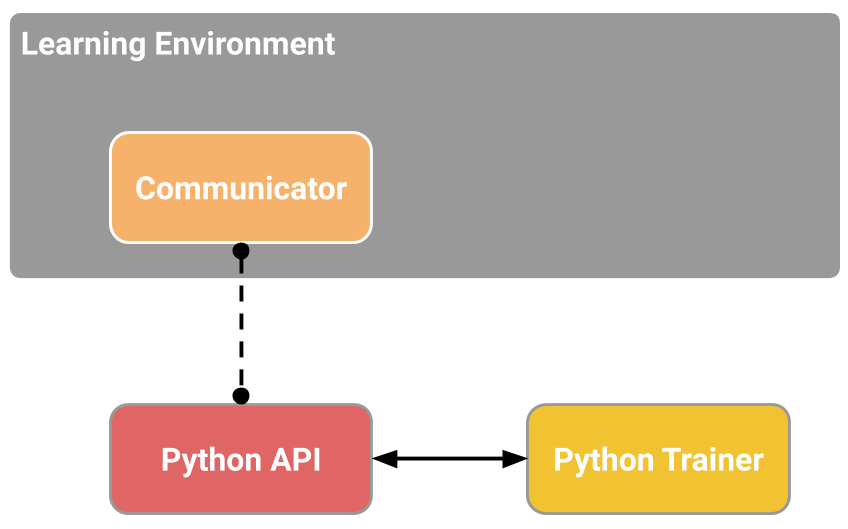
\includegraphics[width = 0.5\textwidth]{Bilder/ml-agents/learning_environment_basic.png}
    \caption{Vereinfachtes Block-Diagramm des ML-Agents-Toolkits \cite{mlagentsOverview}}
    \label{fig:learning-environment-basic}
\end{figure}

Die Trainingsumgebung wird durch zwei enthaltene Unity-Komponenten organisiert \cite{mlagentsOverview}.
\begin{itemize}
    \item \textbf{Agents} sind an ein Unity GameObject geknüpft (beliebiger Charakter innerhalb einer Szene).
    Sie sind gleichzusetzen mit dem Agent eines Reinforcement Learning Problems.
    Agents generieren die Observations (Beobachtungen) des GameObjects, welche dem Reinforcement Learning Algorithmus zugeführt werden, führen die vom Algorithmus empfangenen Aktionen aus und weisen den Reward zu.
    Jeder Agent ist mit einem Behavior verknüpft.

    \item \textbf{Behaviors} (Verhalten) definieren Attribute des Agenten, so auch die Anzahl der Aktionen, die der Agent entgegennehmen kann.
    Ein Behavior kann als Funktion verstanden werden, welche Observations und Reward des Agents als Eingabeparameter enthält und auszuführende Aktionen zurückliefert.
    Behaviors werden in drei Typen unterschieden: \emph{Learning}, \emph{Heuristic} und \emph{Inference}.
    Learning Behaviors sind noch nicht definiert, können aber trainiert werden.
    Heurisitc Behaviors werden mittels manuell implementierter Regeln im Quellcode definiert.
    Inference Behavior werden von trainierten Neural-Network-Dateien (entsprechen der finalen, trainierten Policy) repräsentiert.
    Nachdem ein Learning Behavior trainiert wurde, wird es zum Inference Behavior.
\end{itemize}
Herausstellenswert hierbei ist, dass ML-Agents die Möglichkeit bietet, mehrere Agents in einer Trainingsumgebung zu platzieren, die jedoch mit demselben Behavior verknüpft sein können.
Dies kann dafür genutzt werden, das Training zu parallelisieren und damit zu beschleunigen.

\subsection{Reinforcement Learning Algorithmen}
Von ML-Agents werden zwei Trainingsalgorithmen bereitgestellt, die sich dem (Deep) Reinforcement Learning zuordnen lassen.
Dies sind \acf{ppo} und \acf{sac} \cite{mlagentsOverview}.
In \cite{waidner.2020} wurden diese Algorithmen bereits verglichen.
\ac{ppo} ist der Standardalgorithmus von ML-Agents, da er sich, verglichen mit vielen anderen Reinforcement Learning Algorithmen, als für den allgemeinen Einsatz besser geeignet gezeigt hat \cite{schulman2017proximal,openaiPPO}.
\ac{ppo} ist ein on-policy Algorithmus.
Das bedeutet, dass in jeder Iteration des Lernvorgangs nur aus Erfahrungen gelernt wird, die mit der aktuellen Version der Policy gesammelt wurden.
\ac{sac} hingegen ist ein off-policy Algorithmus und lernt somit aus allen Erfahrungen, die er jemals während des gesamten Trainingsvorgangs gesammelt hat \cite{suran2020,sagar2020}.
Daraus ergeben sich für beide Algorithmen unterschiedliche Vor- und Nachteile.
On-policy Algorithmen haben in der Regel einen deutlich stabileren Lernfortschritt, als off-policy Algorithmen.
Andererseits brauchen on-policy Algorithmen in der Regel deutlich mehr Trainingsschritte, um nennenswerte Ergebnisse zu erzielen \cite{mlagentsOverview}.
Im Zuge der Vorgängerarbeit wurde mit beiden Algorithmen gearbeitet, mit dem Ergebnis, dass der \ac{ppo}-Algorithmus auch für das konkrete Problem im Rahmen dieser Studienarbeit deutlich bessere Resultate liefert \cite[48]{waidner.2020}.

\subsection{Hyperparameter}


\subsection{Bewertungskriterien?}
Value Loss
stetiges Training
\cite{aurelian2018,untiyMetrics}

\section{Beschreibung der Projektbasis}

\section{Vektorgeometrie}
Abstandsbestimmung und Winkel zwischen Vektoren